 \documentclass[oneside,a4paper]{book}
%\pagestyle{headings}
% $Author: oscar $
% $Date: 2009-11-06 14:37:12 +0100 (Fri, 06 Nov 2009) $
% $Revision: 29604 $
%=============================================================
% ST80 listings macros
% Adapted from Squeak by Example book
%=============================================================
% If you want >>> appearing as right guillemet, you need these two lines:
%\usepackage[T1]{fontenc}
%\newcommand{\sep}{\mbox{>>}}
% Otherwise use this:
\newcommand{\sep}{\mbox{$\gg$}}
%=============================================================
%:\needlines{N} before code block to force page feed
\usepackage{needspace}
\newcommand{\needlines}[1]{\Needspace{#1\baselineskip}}
%=============================================================
%:Listings package configuration for ST80
\usepackage[english]{babel}
\usepackage{amssymb,textcomp}
\usepackage{listings}
% \usepackage[usenames,dvipsnames]{color}
\usepackage[usenames]{color}
% \definecolor{source}{gray}{0.95}
\lstdefinelanguage{Smalltalk}{
%  morekeywords={self,super,true,false,nil,thisContext}, % This is overkill
  morestring=[d]',
  morecomment=[s]{"}{"},
  alsoletter={\#:},
  escapechar={!},
  literate=
    {BANG}{!}1
    {UNDERSCORE}{\_}1
    {\\st}{Smalltalk}9 % convenience -- in case \st occurs in code
    % {'}{{\textquotesingle}}1 % replaced by upquote=true in \lstset
    {_}{{$\leftarrow$}}1
    {>>>}{{\sep}}1
    {^}{{$\uparrow$}}1
    {~}{{$\sim$}}1
    {-}{{\sf -\hspace{-0.13em}-}}1  % the goal is to make - the same width as +
    {+}{\raisebox{0.08ex}{+}}1		% and to raise + off the baseline to match -
    {-->}{{\quad$\longrightarrow$\quad}}3
	, % Don't forget the comma at the end!
  tabsize=4
}[keywords,comments,strings]

\definecolor{source}{gray}{0.95}

\lstset{language=Smalltalk,
	basicstyle=\sffamily,
	keywordstyle=\color{black}\bfseries,
	% stringstyle=\ttfamily, % Ugly! do we really want this? -- on
	mathescape=true,
	showstringspaces=false,
	keepspaces=true,
	breaklines=true,
	breakautoindent=true,
	backgroundcolor=\color{source},
	lineskip={-1pt}, % Ugly hack
	upquote=true, % straight quote; requires textcomp package
	columns=fullflexible} % no fixed width fonts
% In-line code (literal)
% Normally use this for all in-line code:
\newcommand{\ct}{\lstinline[mathescape=false,backgroundcolor=\color{white},basicstyle={\sffamily\upshape}]}
% In-line code (latex enabled)
% Use this only in special situations where \ct does not work
% (within section headings ...):
\newcommand{\lct}[1]{{\textsf{\textup{#1}}}}
% Code environments
\lstnewenvironment{code}{%
	\lstset{%
		% frame=lines,
		frame=single,
		framerule=0pt,
		mathescape=false
	}
}{}

% Useful to add a matching $ after code containing a $
% \def\ignoredollar#1{}
%=============================================================
 %seems to create a problem with the preamble command needline already defined

%=============================================================================

\usepackage{amsthm}
\usepackage{xspace}
\usepackage{float}
\usepackage{ifthen}
\usepackage{amsbsy}
\usepackage{amssymb}
\usepackage{balance}
\usepackage{booktabs}
\usepackage{graphicx}
\usepackage{rotating}
\usepackage{multirow}
\usepackage{needspace}
\usepackage{microtype}
\usepackage{bold-extra}
\usepackage{geometry}
\usepackage{varioref}
\usepackage{xcolor}
\usepackage{textcomp}
\usepackage{listings}
\usepackage[normalem]{ulem} %emphasize still italic
\usepackage{ucs}

% \usepackage[utf8]{inputenc}
% \usepackage[htt]{hyphenat}
\usepackage{times}
\usepackage{url}
\usepackage{alltt}
\usepackage{amsmath}
\usepackage{xfrac}
\usepackage{subfigure}
\usepackage{appendix}
\usepackage{stmaryrd}   % for the \shortuparrow
\usepackage[utopia]{quotchap}

\usepackage{setspace}
\usepackage[numbers, sort&compress]{natbib}
\usepackage{mdwlist}        % support for better spaced lists
% allows for temporary adjustment of side margins
\usepackage{chngpage}
\usepackage[normalem]{ulem} 

\usepackage{adjustbox}
\usepackage{verbatim}

% constants

\newcounter{qcounter}

% commands
\newcommand{\n}{$\cdot$}
\newcommand{\y}{\checkmark}
\newcommand{\subscript}[1]{$_{\textrm{\footnotesize{#1}}}$}
\newcommand{\superscript}[1]{$^{\textrm{\footnotesize{#1}}}$}
\newcommand{\vertical}[1]{\raisebox{-4em}{\begin{sideways}{#1}\end{sideways}}}

\newboolean{showedits}
\setboolean{showedits}{true} % toggle to show or hide edits
\ifthenelse{\boolean{showedits}}
{
       \newcommand{\ugh}[1]{\textcolor{red}{\uwave{#1}}} % please rephrase
       \newcommand{\ins}[1]{\textcolor{blue}{\uline{#1}}} % please insert
       \newcommand{\del}[1]{\textcolor{red}{\sout{#1}}} % please delete
       \newcommand{\chg}[2]{\textcolor{red}{\sout{#1}}{\ra}\textcolor{blue}{\uline{#2}}} % please change
	\newcommand{\brs}[1]{\textcolor{orange}{\textbf{\textit{BS:}}#1}}
	\newcommand{\todo}[1]{\textcolor{red}{\textbf{\textit{TODO:}}#1}}
	\newcommand{\meta}[1]{\textcolor{blue}{\textbf{\textit{META:}}#1}}
	\newcommand{\idea}[1]{\textcolor{green}{\textbf{\textit{IDEA:}}#1}}
}{
       \newcommand{\ugh}[1]{#1} % please rephrase
       \newcommand{\ins}[1]{#1} % please insert
       \newcommand{\del}[1]{} % please delete
       \newcommand{\chg}[2]{#2}
}


% ============================================================================
% Put edit comments in a really ugly standout display

\usepackage{xcolor}
\usepackage[normalem]{ulem}
\newcommand{\ra}{$\rightarrow$}


% comments \nb{label}{color}{text}
\newboolean{showcomments}
\setboolean{showcomments}{true}
\ifthenelse{\boolean{showcomments}}
    {\newcommand{\nb}[3]{
        {\colorbox{#2}{\bfseries\sffamily\scriptsize\textcolor{white}{#1}}}
        {\textcolor{#2}{\sf\small$\blacktriangleright$\textit{#3}$\blacktriangleleft$}}}
     \newcommand{\version}{\emph{\scriptsize$-$Id$-$}}
%	 \newcommand{\ugh}[1]{\textcolor{red}{\uwave{#1}}} % please rephrase
%	 \newcommand{\ins}[1]{\textcolor{blue}{\uline{#1}}} % please insert
%	 \newcommand{\del}[1]{\textcolor{red}{\sout{#1}}} % please delete
%	 \newcommand{\chg}[2]{\textcolor{red}{\sout{#1}}{\ra}\textcolor{blue}{\uline{#2}}} % please change
	 \newcommand{\chk}[1]{\textcolor{ForestGreen}{#1}} % changed, please check
	}
    {\newcommand{\nb}[3]{}
     \newcommand{\version}{}
	\newcommand{\chk}[1]{} % changed, please check
	}

% ============================================================================
% Make quotes be italic
\renewenvironment{quote}
    {\list{}{\rightmargin\leftmargin}%
     \item\relax\begin{it}}
    {\end{it}\endlist}

\newcommand{\ttimes}{\ensuremath{\times}}

%=============================================================================

%\newcommand{\needlines}[1]{\Needspace{#1\baselineskip}}

% source code
\usepackage{xcolor}
\usepackage{textcomp}
\usepackage{listings}
\definecolor{source}{gray}{0.9}
\lstset{
	language={},
	% characters
	tabsize=3,
	upquote=true,
	escapechar={!},
	keepspaces=true,
	breaklines=false,
	alsoletter={:},
	breakautoindent=true,
	columns=fullflexible,
	showstringspaces=false,
	basicstyle=\footnotesize\ttfamily,
	% background
	frame=single,
    framerule=0pt,
	backgroundcolor=\color{source},
	% numbering
	numbersep=5pt,
	numberstyle=\tiny,
	numberfirstline=true,
	% captioning
	captionpos=b,
	numberbychapter=false,
	% formatting (html)
	moredelim=[is][\textbf]{<b>}{</b>},
	moredelim=[is][\textit]{<i>}{</i>},
	moredelim=[is][\uline]{<u>}{</u>}}
%\newcommand{\ct}{\lstinline[backgroundcolor=\color{white},basicstyle=\footnotesize\ttfamily]}
%\newcommand{\lct}[1]{{\small\tt #1}}


%----------------------------------------------------------------------------
% references
\newcommand{\tabref}[1]{\hyperref[{tab:#1}]{Table~\ref*{tab:#1}}}
\newcommand{\figref}[1]{\hyperref[{fig:#1}]{Figure~\ref*{fig:#1}}}
\newcommand{\secref}[1]{\hyperref[{sec:#1}]{Section~\ref*{sec:#1}}}
\newcommand{\lstref}[1]{\hyperref[{lst:#1}]{Listing~\ref*{lst:#1}}}
\newcommand{\charef}[1]{\hyperref[{cha:#1}]{Chapter~\ref*{cha:#1}}}
%----------------------------------------------------------------------------

% abbreviations
\tracingcolors 4
\setcounter{tocdepth}{3}
\setcounter{secnumdepth}{3}
\newcommand{\ie}{\emph{i.e.,}\xspace}
\newcommand{\eg}{\emph{e.g.,}\xspace}
\newcommand{\etc}{\emph{etc.}\xspace}
\newcommand{\etal}{\emph{et al.}\xspace}


\newcommand{\newevenside}{
	\ifthenelse{\isodd{\thepage}}{\newpage}{
	\newpage
        \phantom{placeholder} % doesn't appear on page
	\thispagestyle{empty} % if want no header/footer
	\newpage
	}
}

\def\stretchfactor{1}
\newcommand{\mychapter}[1]{\setstretch{1}
    \chapter{#1}\setstretch{\stretchfactor}}

%----------------------------------------------------------------------------
\newcommand{\lessSpace}{\vspace{-1em}}
\DeclareGraphicsExtensions{.pdf,.png}
\graphicspath{{images/}}
\newcommand{\fig}[4]{
	\begin{figure}[#1]
		\centering
		\includegraphics[width=#2\textwidth]{#3}
		\lessSpace
		\caption{\label{fig:#3}#4}
	\end{figure}}

% ===========================================================================

%:CONFIGURE THIS

\newcommand{\thesistitle}{TestView Plugin}
\newcommand{\thesisauthor}{Dominic Sina}
\newcommand{\thesisauthorOrigin}{Zollikofen BE, Switzerland}
\newcommand{\thesisleiter}{Prof.\ Dr.\ Oscar Nierstrasz}
\newcommand{\thesisasst}{Boris Spasojevi\'c}
\newcommand{\thesisurl}{http://scg.unibe.ch/}
\newcommand{\thesissubtitle}{A Nautilus Plugin to facilitate Unit Testing}
\newcommand{\thesisdate}{05. Februar 2015}

% ===========================================================================

\usepackage[ colorlinks=true, urlcolor=black, linkcolor=black,
			citecolor=black, bookmarksnumbered=true, bookmarks=true,
			plainpages=false,
			pdftitle={\thesistitle}, pdfauthor={\thesisauthor},
			pdfsubject={\thesissubtitle}, pdfpagelabels]{hyperref}

\newcommand{\hrref}[2]{\hyperref}
% ===========================================================================
% ===========================================================================


% D O C U M E N T
% % % % % % % % % % % % % % % % % % % % % % % % % % % % % % % % % %
\begin{document}

% T I T L E
% % % % % % % % % % % % % % % % % % % % % % % % % % % % % % % % % %
\begin{titlepage}  
  \begin{center}  
  
  \begin{figure}[t]  
  \vspace*{-2cm}        % to move header logo at the top 
  \center{
\includegraphics[scale=0.5]{logos/UNI_Bern.png}}
  \vspace{1.2in}     
  \end{figure}

    \thispagestyle{empty}
    
    {\bfseries\Huge \thesistitle \par
    \Large \vspace{0.1in} \thesissubtitle \par}

    \vspace{0.3in} 
    \LARGE{\textbf{Bachelor Thesis} \\}
    \vspace{0.4in}

    {\Large \thesisauthor \par from \par \thesisauthorOrigin}
    
    \vspace{0.3in}
    {\Large Philosophisch-naturwissenschaftlichen Fakult\"{a}t \\
            der Universit\"{a}t Bern \par}
    \vspace{0.3in}
    {\Large \thesisdate \par}
    \vspace{0.3in}
    %Leiter der Arbeit: \par
   {\Large \thesisleiter} \par
      {\Large \thesisasst} \par
   \vspace{0.1in}
    {\Large Software Composition Group \par Institut f\"{u}r Informatik und angewandte Mathematik \par University of Bern, Switzerland \par}
  

  %\vspace{0.5in}
 
 

  \end{center}

\end{titlepage}



% A B S T R A C T
% % % % % % % % % % % % % % % % % % % % % % % % % % % % % % % % % %
\chapter*{\centering Abstract}
	\begin{quotation}
		\noindent 
The purpose of this bachelor project is to improve the Pharo enviroment by making it more unit test friendly. 
Instead of writing a new system browser we chose to realise this in the form of a Nautilus plugin since this makes it easy to set up and builds on an established part of the Pharo enviroment. Our plugin's functions includes making it easier to creating new tests for a given method. Specifically being able to see a method and the test that is currently being written side by side and a fast way to create new tests with if necessary new test classes and packages. The second provided functionality is a search for existing tests corresponding to the currently selected method. The search takes in to account if the methods are similarly named, if the supposed test method is a subclass of TestCase and if it contains the selector of the original method. The user can then add and remove elements from the resulting collection of tests to ensure that only acctual tests are shown. These features not only facilitate unit testing but can also be used to help understanding methods by looking at their tests.  
	\end{quotation}
\clearpage


% C O N T E N T S 
% % % % % % % % % % % % % % % % % % % % % % % % % % % % % % % % % % % % % % % %
\tableofcontents

%%%%%%%%%%%%%%%%%%%%%%%%%%%%%%%%%%
%%%% Introduction %%%%%%%%%%%%%%%%%%%%%
%%%%%%%%%%%%%%%%%%%%%%%%%%%%%%%%%%
\chapter{Introduction}
	\label{cha:introduction}

\section{Unit Testing}
	\label{sec:Unit Testing}
The TestView plugin was designed with this approach to testing in mind. Unit testing follows the paradigm of isolation the smallest inseparable part of a programm and testing it. In smalltalk these units are often methods since the language heavily relies on sending messages between object. Also implied with this approach is that the programm is already written when the tests are written. The plugin helps during the creation of each test since the user can easily view the the tested method as well as the test that is being written. Further it creates templates that the user can alter to make writting tests faster. I also helps finding existing test and thus finding methods without tests. This functionaly however is at the moment not automated and the user will have to select method after method to find those without tests.  
	\begin{enumerate}
		\item Designed with this in mind
		\item Method first, test later
		\item Looking at both method and test being written
		\item Facilitate creating tests
	\end{enumerate}

\section{Test-driven Development}
	\label{sec:Test-driven Development}
	\begin{enumerate}
		\item Hard to do with this plugin
		\item Test first, method later
		\item Search mechanism searches tests for methods
		\item When creating a test it can not be linked to a class since the class doesn't exist yet 
		\item Helps adapting tests to methods if requirements change or during development problems with the orignal tests show up		
	\end{enumerate}

\section{The Nautilus Plugin Framework}
	\label{sec:The Nautilus Plugin Framework}


%%%%%%%%%%%%%%%%%%%%%%%%%%%%%%%%%%
%%%% Related work %%%%%%%%%%%%%%%%%%%%%
%%%%%%%%%%%%%%%%%%%%%%%%%%%%%%%%%%
\chapter{Related Work}
	\label{cha:Related Work}
In which we learn what have other done to address similar problems. For example, the work of Star \cite{Star89}
\\eclipse
\\-easy to view multiple methods at once
\\-no automated testsearch
\\Nautilus/pharo
\\-automated testsearch is a bit lacking but exists (doesn't support multiple tests for one method<-check if true)
\\-no easy way to view multiple methods
\\--history droplist can't be used when user klicks on too many classes/methods
\\--could open another Nautilus window but dublicate package tree takes up a lot of space
\\--best solution so far: lock method, then navigate to testmethod or write new test (but multipleMethodEditor is kinda broken)


%%%%%%%%%%%%%%%%%%%%%%%%%%%%%%%%%%
%%%% The Problem %%%%%%%%%%%%%%%%%%%%%
%%%%%%%%%%%%%%%%%%%%%%%%%%%%%%%%%%
\chapter{The Problem}
	\label{cha:The Problem}
%put some direct references to problems in the environments mentioned above
 As seen in the examples many current development environments are not optimized for unit testing. The search for unit tests to a specific method is often lacking meaning not present or simplistic and not able to recognize multiple tests for one method. Important features for unit test friendly environments are automated test searching, the ability to view tests and methods side by side and the ability to easily create new tests. Since not many environments were created with specificaly unit testing in mind there are often some of these features missing. To compensate for this the user is required to manualy execute many tasks like for example navigating back and forth between method and test and creating new classes and packages for new tests. This repeatedly breaks the programmers flow and in effect discourages them from writting tests. \\ \par

Taking a closer look at the tasks involved in different goals will help understanding the problem of those missing functionalities and exactly at which point they are needed. A very important feature for unit testing is the ability to see which methods are currently untested. This has to be as easy to see as possible to be really beneficial. The user should be able to determine with one glance which methods have no tests. If this feature is not implemented the user has to switch back and forth between a class and all its test classes to check. If the test classes are not known to them they even have to find them first. Both of those tasks can take alot of effort. \\ \par

Similarly the user might want too see all the tests that have been written for a method and not just if it has tests at all. This not only helps the user decide if it is necessary to write a specific test or if a very similar test has already been created but also lets them view how methods work by looking at all their tests. \\ \par

Another reoccuring goal is the creation of new test for methods with no or too less tests. 
While creating a new test the user first has to decide in which package and class the new test will be added. In many cases it is already clear where the test will be located since other tests corresponding to the same method are already there. If there are no already existing tests or if for any reason the existing test classes do not fit the new test then the user has to create a new test. In this case the test package name and the test class name are often derived from the original package and class. Both of those should be set as default values for the new class and package to save some time. When writting the actual code for the test it is beneficial for the user to be able to see test and method side by side. With this it the user is able to easily do white-box testing. For black-box testing this feature is less important but if it can be easily turned off it should not interfere. Similarly as above this helps preventing the user switching back and forth between methods.\\  \par
 
These examples show where problems can occour that hinder the user while doing unit testing. They increase the time and effort needed and to create unit tests and thus make writing tests a chore. By facilitating this process on the other hand the user is encouraged to write tests and hopefully increase the quality of the software that is being written.

%%%%%%%%%%%%%%%%%%%%%%%%%%%%%%%%%%
%%%% The TestView Plugin %%%%%%%%%%%%%%%%%%%%%
%%%%%%%%%%%%%%%%%%%%%%%%%%%%%%%%%%
\chapter {The TestView Plugin}
	\label{cha:The TestView Plugin}
In this chapter the TestView plugin is explainded. The first section will show how to install the plugin while the following ones will go over what the visual components do and explain the inner workings of the plugin, namely how test are found and how they can be created using the plugin.

\section{Installation and activation}
	\label{sec:Installation and activation}
To install and active the TVPlugin follow the steps listed bellow:
	
	\begin{enumerate}

		\item To download the necessary packages simply simply execute the following lines in a Pharo workspace \begin{code}Gofer new
url: 'http://smalltalkhub.com/mc/DominicSina/TestView/main';
package: 'ConfigurationOfTestView';
load.
(Smalltalk at: #ConfigurationOfTestView) loadDevelopment.
NautilusPluginManager new openInWorld\end{code} 
Once this is finished the Nautilus Plugins Manager will open. 	
	
		\item Here you click on "TVPlugin" under "Available plugin classes" and then press on the "Add" button. In the "Selected plugins" collumn you can specify where most visual elements will be shown in your Nautilus windows. Click "Ok" to confirm.
			\begin{center}
				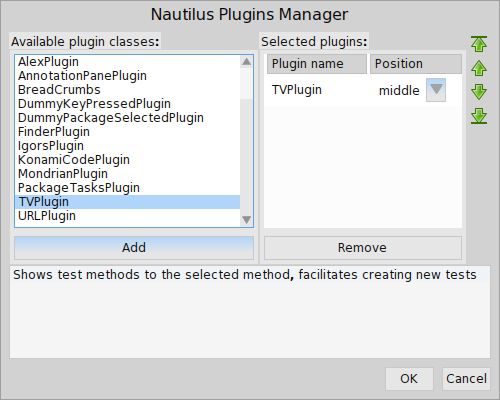
\includegraphics[scale=0.4]{screenshots/pluginManager.png}
			\end{center}

		\item When you open a Nautilus window from now on the plugin will be started until you remove it again using the Nautilus Plugins Manager. To verify if the plugin is activated check if this row is displayed in the position you selected.
			\center{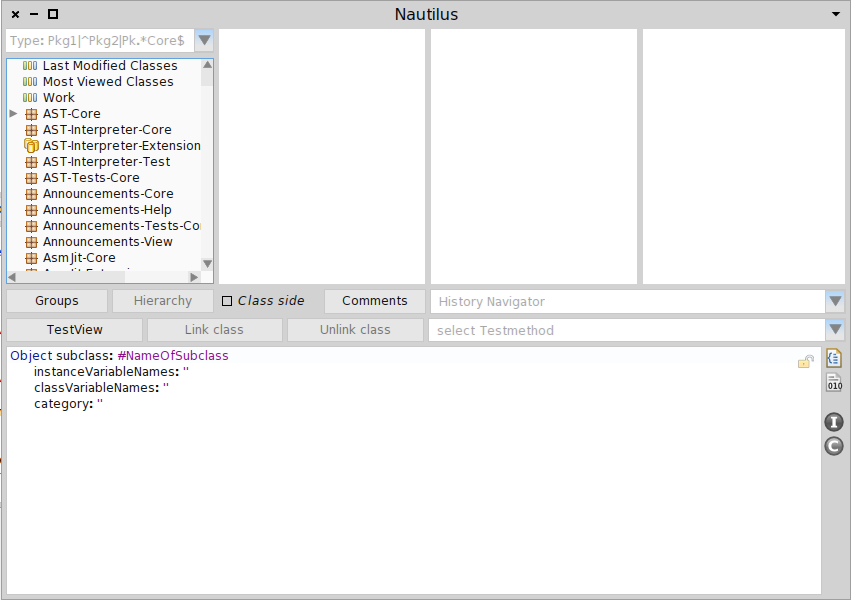
\includegraphics[scale=0.5]{screenshots/activatedPlugin.png}}
	\end{enumerate}



\section{Basic Components}
	\label{sec:Basic Components}
Here a quick overview of all the visiual elements can be found. The TVPlugin adds 3 buttons and one droplist to your Nautilus windows. The "TestView" button toggles the search for test methods to the currently selected method. If it is toggled on a second source code editor will appear at the bottom where the test methods will be displayed. This list will change whenever a new method is selected in the Nautilus window.
The initial list shown in the droplist is composed of tests found through the search algorithm described under \ref{sec:The search Algorithm} \nameref{sec:The search Algorithm}. The additional buttons "Link Class" and "Unlink Class" allow to customise this list if the search for any reason did not find some tests.

\section{The search Algorithm}
	\label{sec:The search Algorithm}
In this section I will provide a detailed explanation how corresponding tests to a certain method are found. It is a hierarchical search with two stages. \\ \par
In the first stage all test classes are determined. For this all classes in the your enviroment are taken into consideration in the beginning. By the end of the first stage only those classes that inherit from "TestCase" as well as pass a substring search in the class name are then passed over to the next step. The substring search requires the name of the class in question to contain both "test" and the name of the selected class. If those two conditions are met then the class in question is a test class of the selected class. The substring search is not case sensitive and the matches for "test" as well as the selected method can't overlap, meaning one letter can only be used to match partially either "test" or the selected class name.\\ \par

\begin{center}
   \begin{tabular}{| l || c | r |}
     \hline
     Original class name & Possible class names & Not a test class name \\ \hline \hline
     String & StringTest, stringtest, TestString & String, Test, StrinTgEST \\ \hline
     Protest & ProtestTest & Protest \\
     \hline
   \end{tabular}
\end{center}

In the second stage all test methods corresponding to the selected method out of all methods of the test classes are determined. Similarly as before the test method name needs to contain the name of the selected method in addition to "test". The second criterion is if the method in question uses the selector of the selected method. Unlike stage one this stage is fairly inclusive in that if only one of those criteria is satisfied it still qualifies as a test to the selected method.\\ \par
The two criteria of the second stage also serve to order the found test methods. The ones displayed on top satisfy both criteria. The ones that only satify the naming requirement are shown below these and the last ones are those that only contain the selector of the selected method. 

\section{Creating new Tests}
	\label{sec:Creating new Tests}
The other main functionality of the plugin besides finding tests is to facilitate creating them. When you have a method open in the first code editor to which you would like to add a test select the "new Test" option from the droplist. This option is an exception to the order discribed at the end of \ref{sec:The search Algorithm} \nameref{sec:The search Algorithm} and is always shown on top of the list. This option also can be found there regardless wheter there were any tests found for the selected method. A template will appear in the second editor where the user can write the new test. When the test is accepted the user will be asked to name the class in which this test will be added. If the specified class doesn't exist it will be created and the user will be asked for a package to place it in. \\ \par 
A faster way to create a new test is to select an existing test from the droplist and alter it. By selecting a new name the old test will not be overwritten and the new test will be added to the class of the old test. Any test that was written using the second editor will result in its class being linked to the class of the selected method. This makes sure that the class in which the test was added is later recognised by the search algorithm even if its name does not confirm to the naming of a test class.

\begin{center}
	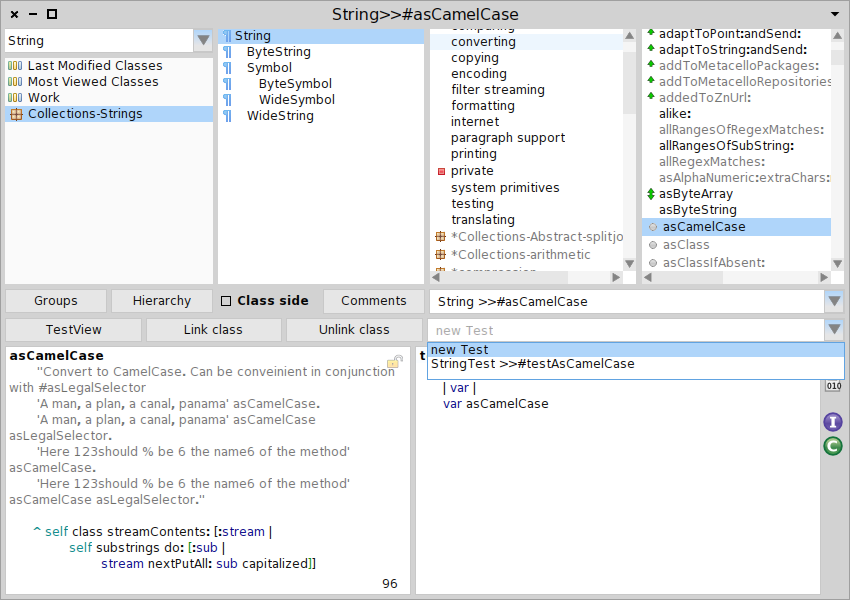
\includegraphics[scale=0.4]{screenshots/dropListOpen.png}
\end{center}

%%%%%%%%%%%%%%%%%%%%%%%%%%%%%%%%%%
%%%% The Validation %%%%%%%%%%%%%%%%%%%%%
%%%%%%%%%%%%%%%%%%%%%%%%%%%%%%%%%%
\chapter {The Validation}
	\label{cha:The Validation}
In which you show how well the solution works.

%%%%%%%%%%%%%%%%%%%%%%%%%%%%%%%%%%
%%%% Conclusion and Future Work %%%%%%%%%%%%%%%%%%%%%
%%%%%%%%%%%%%%%%%%%%%%%%%%%%%%%%%%
\chapter {Conclusion and Future Work}
	\label{cha:Conclusion and Future Work}
In which we step back, have a critical look at the entire work, then conclude, and learn what lays beyond this thesis.

%%%%%%%%%%%%%%%%%%%%%%%%%%%%%%%%%%
%%%% Anleitung zu wissenschaftlichen Arbeiten %%%%%%%%%%%%%%%%%%%%%
%%%%%%%%%%%%%%%%%%%%%%%%%%%%%%%%%%
\chapter {Anleitung zu wissenschaftlichen Arbeiten}
	\label{cha:Anleitung zu wissenschaftlichen Arbeiten}
This consists of additional documentation, e.g. a tutorial, user guide etc.
Required by the Informatik regulation.

%END Doc
%-------------------------------------------------------

\bibliography{thesis}
\bibliographystyle{plain}

\end{document}